%%%%%%%%%%%%%%%%%%%%%%%%%%%%%%%%%%%%%%%%%%%%%%%%%%%%%%%%%%%%%%%%%%%%%%%%

%%% LaTeX Template for ECAI Papers 
%%% Prepared by Ulle Endriss (version 1.0 of 2023-12-10)

%%% To be used with the ECAI class file ecai.cls.
%%% You also will need a bibliography file (such as mybibfile.bib).

%%%%%%%%%%%%%%%%%%%%%%%%%%%%%%%%%%%%%%%%%%%%%%%%%%%%%%%%%%%%%%%%%%%%%%%%

%%% Start your document with the \documentclass{} command.
%%% Use the first variant for the camera-ready paper.
%%% Use the second variant for submission (for double-blind reviewing).

\documentclass{ecai} 

%\documentclass[doubleblind]{ecai} 

%%%%%%%%%%%%%%%%%%%%%%%%%%%%%%%%%%%%%%%%%%%%%%%%%%%%%%%%%%%%%%%%%%%%%%%%

%%% Load any packages you require here. 

\usepackage{latexsym}
\usepackage{amssymb}
\usepackage{amsmath}
\usepackage{amsthm}
\usepackage{booktabs}
\usepackage{enumitem}
\usepackage{graphicx}
\usepackage{color}

\usepackage[T1]{fontenc}
\usepackage{graphicx}
%\usepackage{color}
%\renewcommand\UrlFont{\color{blue}\rmfamily}

\usepackage{amsmath,amssymb,amsfonts}
% \usepackage[inline, shortlabels]{enumitem}
\usepackage{tabularx}
\usepackage{caption}
% \usepackage{titlesec}
\usepackage[english]{babel}
\captionsetup{font=it}
\usepackage{ragged2e}
\usepackage{hyperref}
\usepackage{pifont}
\usepackage{footmisc}
\usepackage{multirow}
\usepackage{algorithm2e}

% --- Tickz
\usepackage{physics}
\usepackage{amsmath}
\usepackage{tikz}
\usepackage{mathdots}
\usepackage{yhmath}
\usepackage{cancel}
\usepackage{color}
\usepackage{siunitx}
\usepackage{array}
\usepackage{multirow}
\usepackage{amssymb}
\usepackage{gensymb}
\usepackage{tabularx}
\usepackage{extarrows}
\usepackage{booktabs}
\usetikzlibrary{fadings}
\usetikzlibrary{patterns}
\usetikzlibrary{shadows.blur}
\usetikzlibrary{shapes}

% ---------

\usepackage{pdfpages}
\usepackage{booktabs}
\usepackage{csquotes}
\usepackage{lipsum}  
\usepackage{arydshln}
\usepackage{smartdiagram}
\usepackage[inkscapeformat=png]{svg}
\usepackage{textcomp}
\usepackage{tabularray}\UseTblrLibrary{varwidth}
\usepackage{xcolor}
\def\BibTeX{{\rm B\kern-.05em{\sc i\kern-.025em b}\kern-.08em
    T\kern-.1667em\lower.7ex\hbox{E}\kern-.125emX}}
% \usepackage{cite}
\usepackage{amsmath}
\newcommand{\probP}{\text{I\kern-0.15em P}}
\usepackage{etoolbox}
\usepackage{listings}
\usepackage{etoolbox}
\patchcmd{\thebibliography}{\section*{\refname}}{}{}{}

%%%%%%%%%%%%%%%%%%%%%%%%%%%%%%%%%%%%%%%%%%%%%%%%%%%%%%%%%%%%%%%%%%%%%%%%

%%% Define any theorem-like environments you require here.

\newtheorem{theorem}{Theorem}
\newtheorem{lemma}[theorem]{Lemma}
\newtheorem{corollary}[theorem]{Corollary}
\newtheorem{proposition}[theorem]{Proposition}
\newtheorem{fact}[theorem]{Fact}
\newtheorem{definition}{Definition}

%%%%%%%%%%%%%%%%%%%%%%%%%%%%%%%%%%%%%%%%%%%%%%%%%%%%%%%%%%%%%%%%%%%%%%%%

%%% Define any new commands you require here.

% \newcommand{\BibTeX}{B\kern-.05em{\sc i\kern-.025em b}\kern-.08em\TeX}

\setlength\tabcolsep{0.5pt}

\newcommand{\before}[1]{\textcolor{red}{#1}}
\newcommand{\after}[1]{\textcolor{green}{#1}}

\newcommand{\old}[1]{\textcolor{orange}{#1}}
\newcommand{\rem}[1]{\textcolor{red}{#1}}
\newcommand{\todo}[1]{\textcolor{orange}{\newline \textit{\textbf{TODO:} #1}} \newline \newline }


\definecolor{codegreen}{rgb}{0,0.6,0}
\definecolor{codegray}{rgb}{0.5,0.5,0.5}
\definecolor{codepurple}{rgb}{0.58,0,0.82}
\definecolor{backcolour}{rgb}{0.95,0.95,0.92}
 
\lstdefinestyle{mystyle}{
    backgroundcolor=\color{backcolour},   
    commentstyle=\color{codegreen},
    keywordstyle=\color{magenta},
    numberstyle=\tiny\color{codegray},
    stringstyle=\color{codepurple},
    basicstyle=\footnotesize,
    breakatwhitespace=false,         
    breaklines=true,                 
    captionpos=b,                    
    keepspaces=true,                 
    numbers=left,                    
    numbersep=5pt,                  
    showspaces=false,                
    showstringspaces=false,
    showtabs=false,                  
    tabsize=2
}
 
\lstset{style=mystyle}


\newcounter{relation}
\setcounter{relation}{0}
\renewcommand{\therelation}{\arabic{relation}}
\newcommand{\relationautorefname}{Relation}

\newenvironment{relation}[1][]{%
    \refstepcounter{relation}%
    \noindent \raggedright \textit{\textbf{Relation. \therelation}} \hfill$}
{%
$ \hfill \phantom{x}

}

\newcounter{proof}
\setcounter{proof}{0}
\renewcommand{\theproof}{\arabic{proof}}
\newcommand{\proofautorefname}{Proof}

\renewenvironment{proof}[1][]{
    \refstepcounter{proof}
    \noindent \raggedright \textit{\textbf{Proof. \theproof}}

    \setlength{\leftskip}{1em}

}
{

\
\setlength{\leftskip}{0pt}
}

%%%%%%%%%%%%%%%%%%%%%%%%%%%%%%%%%%%%%%%%%%%%%%%%%%%%%%%%%%%%%%%%%%%%%%%%

\begin{document}

%%%%%%%%%%%%%%%%%%%%%%%%%%%%%%%%%%%%%%%%%%%%%%%%%%%%%%%%%%%%%%%%%%%%%%%%

\begin{frontmatter}

    %%% Use this command to specify your submission number.
    %%% In doubleblind mode, it will be printed on the first page.

    \paperid{123}

    %%% Use this command to specify the title of your paper.

    \title{A Library for Helping Explainable MARL with Organizational Models}

    % JS: keywords:
    %     Multi-Agent Reinforcement Learning
    %     Explainability
    %     Organizational Models
    %     Cooperative Intelligence

    %%% Use this combinations of commands to specify all authors of your 
    %%% paper. Use \fnms{} and \snm{} to indicate everyone's first names 
    %%% and surname. This will help the publisher with indexing the 
    %%% proceedings. Please use a reasonable approximation in case your 
    %%% name does not neatly split into "first names" and "surname".
    %%% Specifying your ORCID digital identifier is optional. 
    %%% Use the \thanks{} command to indicate one or more corresponding 
    %%% authors and their email address(es). If so desired, you can specify
    %%% author contributions using the \footnote{} command.

    \author[A,B]{\fnms{Julien}~\snm{Soulé}\thanks{Corresponding Author. Email: julien.soule@lcis.grenoble-inp.fr}}
    \author[A]{\fnms{Jean-Paul}~\snm{Jamont}}
    \author[A]{\fnms{Michel}~\snm{Occello}}
    \author[B]{\fnms{Louis-Marie}~\snm{Traonouez}}
    \author[C]{\fnms{Paul}~\snm{Théron}}

    \address[A]{Univ. Grenoble Alpes, Grenoble INP, LCIS, 26000, Valence, France}
    \address[B]{Thales Land and Air Systems, BL IAS, Rennes, France}
    \address[C]{AICA IWG, La Guillermie, France}

    %%% Use this environment to include an abstract of your paper.

    \begin{abstract}
        % Context
        The MAS organization can be seen both from the point of view of individual agents' interactions or through the collective patterns at a global level. Searching for an organization that allows achieving a goal under given or environmental constraints is central in MAS design.
        %
        % Issue
        An empirical approach to finding a suitable organization in some environments can be costly.
        %
        % Contribution
        We propose PRAHOM which augments the PettingZoo simulation framework to suggest organizational specifications likely to guide the design towards a suitable MAS.
        It integrates constraints into learning and generates organizational specifications using the trained agents' behaviors.
        % The generated specifications can guide the designers.
    \end{abstract}

\end{frontmatter}

%%%%%%%%%%%%%%%%%%%%%%%%%%%%%%%%%%%%%%%%%%%%%%%%%%%%%%%%%%%%%%%%%%%%%%%%

\section{Introduction}

% Context:


%% Introduce the concept of Cyberdefense SMA by supporting it by the AICA
% Introduce the problem of SMA design in general from this specific case


% An AICA agent~\cite{Kott2023}
%
% (\emph{Autonomous Intelligent Cyberdefense Agent}\footnote{Research on AICAs was initiated within the framework of the \emph{NATO IST-152} group then the \emph{AICA International Work Group}: \url{ https://www.aica-iwg.org/}.})
% %
% must be deployed in a networked environment to detect, identify, characterize attacks, develop and execute countermeasures to minimize potential damage.
% An AICA agent can be seen as a Cyberdefense SMA~\cite{Singh2015} where Cyberdefense coverage is distributed over a set of Cyberdefense agents collaborating with each other autonomously.

% todo

%\jp{I don't like this attack on the article... it's abrupt... we're talking about it}
% js: Our contribution addresses the problem of design...
%jpj I didn't say it was necessary, I said it's abrupt
% js: ok so I keep it like this? at least it's clear even if it's not very nicely written
%no Michel doesn't like it either: we talked about it yesterday in a meeting
% wait let me read the article I can't ignore your comments :) and I'll start again
% js: ok, I don't touch and will you send me a message when you're finished?
The design of an MAS requires that the designer have knowledge of the deployment environment in order to propose internal logic to the agents likely to allow them to collectively achieve the given objective.
%
This knowledge may prove insufficient due to the complexity of the environment; or due to access constraints (temporal, spatial and legal) limiting the possibilities of its empirical understanding.
% \jp{metaproposal: The design of an SMA requires having a good knowledge of the deployment environment because... . In many applications in particular... the environment is....}
% The flexibility of a Cyberdefense SMA strengthens its resilience by allowing it to continually adapt to environmental constraints while respecting security policies. Organizational aspects are considered in the engineering of such an MAS within the research work.

%% Broaden the subject of SMAC/AICA to the context of SMA in general

% \jp{check that it makes sense after reformulating "this problem"}
Designing an MAS can be seen through the \textbf{organization} which we see as the set of \textbf{policies} of the agents
\footnote{A policy is a relationship between observations and actions.}
considered both from an individual point of view and from a global point of view. The organizational mechanisms induced by these policies can be explained through \textbf{organizational models}.

% \jp{Question that will arise: we say that we do not know (or very poorly) the environment and therefore we are learning on a simulated environment}


% the \textbf{organizational support} which explains how agents coordinate their activities to collaboratively achieve a common objective.
The design of an SMA then becomes the search for an organization allowing the given objective to be achieved optimally under environmental constraints.
\footnote{Approach developed in the article \textquote{An Approach based on Reinforcement Learning for the Organizational Engineering of an SMA} submitted for JFSMA 2024 }.
Even if most design methods such as GAIA~\cite{Cernuzzi2014} or KB-ORG~\cite{Sims2008} facilitate the search for an adequate organization for a given environment and objective~\cite{Mefteh2013}; they do not make it possible to completely automate the search for agent policies satisfying the given requirements and explaining the organization.

We introduce \emph{PRAHOM Wrapper} (Partial Relations with Agent History and Organization Model Wrapper), a software layer for the Multi-Agent simulation framework \emph{PettingZoo} which allows to:
%
i) Train agent policies to achieve a given objective in an environment and while respecting possible organizational specifications;\quad
ii) Determine organizational specifications %\MO: from%
by analyzing the behavior of trained agents.
%
% \jp{you say "aim" whose objective but it is not the objective that you give here it is the means}
To do this, it combines a MARL (Multi-Agent Reinforcement Learning) process with the $\mathcal{M}OISE^+$~\cite{Hubner2007} organizational model.

% Section II first summarizes the fundamental concepts on which \emph{PRAHOM Wrapper} is built.
Section II provides an overview of the positioning of \emph{PRAHOM Wrapper} among existing works.
Section III presents the functionalities offered by \emph{PRAHOM Wrapper} and its use in an Atari game type environment.
Section IV concludes on \emph{PRAHOM Wrapper} by discussing its limitations and future work.

% ==================================================== = ==================================================== == =

% \section{Fundamental Concepts}

% We present the bases of the $\mathcal{M}OISE^+$ organizational model and the MARL bases on which \emph{PRAHOM Wrapper} is built.

% \subsection{Organizational model $\mathcal{M}OISE^+$}

% $\mathcal{M}OISE^+$~\cite{Hubner2007} makes it possible to characterize an organization according to three types of specifications:

% \textbf{structural specifications} describe the means that agents can exploit to achieve an objective. It includes all \emph{roles}, subgroups, intra- and inter-group \emph{links}, intra- and inter-group \emph{compatibilities}, as well as the \emph {cardinalities} of the roles and subgroups.
% % A \emph{link} indicates whether two roles are linked due to ties of knowledge, communication, or authority. A \emph{compatibility} indicates whether two roles can be adopted by the same agent. Role and subgroup \emph{cardinalities} refer to the minimum and maximum number of roles and subgroups, respectively.

% \textbf{functional specifications} describe how to achieve a goal. It includes, among other things, global \emph{objectives}, \emph{missions}, \emph{plans} and the cardinality of the agents engaged in a mission.

% \textbf{deontic specifications} make it possible to link functional and structural specifications through a set of \emph{permissions} and \emph{obligations} during specific periods.
% % A \emph{permission} means that an agent playing the role $\rho_a$ is authorized to engage in the mission $m$ for a given time constraint $tc$. Likewise, an \emph{obligation} means that an agent playing the role $\rho_a$ must commit to the mission $m$ for a given time constraint $tc$. A time constraint $tc$ specifies a set of periods determining whether an authorization or obligation is valid.


% \subsection{Multi-agent Reinforcement Learning}

% This pushes agents to converge towards cooperation mechanisms, collective strategies, etc.

% We use the Markov model \emph{Dec-POMDP} (Decentralized-Partially Observable Markov Decision Process)~\cite{Oliehoek2016} to model an environment and apply MARL techniques. Indeed, it considers several agents in a way similar to an MAS. It makes it possible to model the uncertainty of the environment for the changes induced by the actions and the observations received. Its reward function is common to agents, which promotes the formation of actions oriented towards collaboration~\cite{Beynier2013}.
% % Formally, a Dec-POMDP is a 7-tuple $(S,\{A_i\},T,R,\{\Omega_i\},O,\gamma)$ , where: $S = \{s_1, .. s_{|S|}\}$ is the set of possible states; $A_{i} = \{a_{1}^{i},..,a_{|A_{i}|}^{i}\}$ the set of possible actions for the agent $i$; $T$ so that $T(s,a,s') = \probP{(s'|s,a)}$ the set of conditional transition probabilities between states; $R: S \times A \times S \rightarrow \mathbb{R}$ the reward function; $\Omega_{i} = \{o_{1}^{i},..,o_{|\Omega_{i}|}^{i}\}$ the set of observations for the agent $ag_i $ ; $O$ so that $O(s',a,o) = \probP{(o|s',a)}$ the set of conditional observation probabilities; $\gamma \in [0,1]$, the discount factor.

% We call \textbf{solve}/\textbf{solve sub-optimally} the Dec-POMDP for a team, the search for a joint policy allowing to maximize/exceed a cumulative reward threshold over a finite horizon.

% % ================================================ ============================

\section{Works and positioning}

ADR is a machine learning paradigm where agents learn to make decisions by interacting with an environment. The goal is for a set of agents to maximize the cumulative reward over time through a process of trial and error.
MARL makes it possible to automatically converge towards policies enabling the given objective to be achieved. Reinterpreting these individual policies into organizational specifications requires work on explainability at a collective level that is rarely addressed in the literature.
% \jp{explainability only or also organizational aspects... if it is both it is necessary to review "the question of organization and in particular of its explainability"}.
% We present the overview of related works identified in three categories.
% I'm making changes to the text: you'll have to reread properly :)

\paragraph{\textbf{Frames for ADR with organizational aspects}}
%
% \jp{verify that AAAAA et al. is very singular}
% \jp{can be started with a sentence that explains what we call the framework for MARL with organizational aspects. The others (the following 2 paragraphs seem more explicit to me}
Some proposed frameworks attempt to include organizational concepts within the ADR framework.
Kazhdan and. al.~\cite{Kazhdan2020} present a library to improve the explainability of MARL systems by bringing them closer to symbolic models, in particular to infer roles.%todo
% \jp if Kazhdan is not interested in organizations it's awkward}
%
Wang et. al.~\cite{Wang2020} introduce an approach in which similar emerging roles are pushed to jointly specialize on specific tasks.
% \jp{the roles specialize themselves ???} jointly.
%
% Tosic et. al~\cite{Tosic2010} proposes a framework for coordination based on the communication capabilities of multi-agent systems.
%
% Zheng et. al.~\cite{Zheng2018} presented a platform for MARL that aims to facilitate research on artificial collective intelligence by providing a comprehensive set of evaluation metrics to compare the performance of MARL algorithms.

\paragraph{\textbf{Characterization of emerging collective strategies}}
%
Heuillet and. al.~\cite{Heuillet2022} propose an approach to explain cooperative strategies using Shapley values. Its effectiveness has been demonstrated in the context of applications on multi-agent particle environments by explaining certain decisions taken.
%
Jaques and. al.~\cite{Jaques2019} propose a mechanism to benefit from communication between agents by rewarding agents having a causal influence on other agents. This approach leads to learned communication protocols allowing for overall more efficient collective behavior.
% \jp{adaptive? pcq in absolute terms a more diversified collective behavior we don't care}.
% js: generally more efficient (see https://arxiv.org/abs/1810.08647)

\paragraph{\textbf{Adaptation of MARL to meet requirements}}
%
% Shao and. al.~\cite{Shao2022} introduces an approach based on the leader-follower model as a mechanism to improve multi-agent cooperative tasks with dynamic characteristics, aiming to improve the adaptability and generalization of ADR systems.
%
% Roy et. al.~\cite{Roy2020} presents two policy regularization methods aimed at improving coordination in reinforcement learning.
% %
\emph{Specification-Guided Reinforcement Learning} aims to generate policies that accomplish a specific task using external specifications to guide learning in achieving an objective and under given constraints~\cite{Bansal2022}.% ~\cite{Jothimurugan2023}%
%\jp{does that mean that it is used for the identification/characterization of SMA?}
%
%
~Jothimurugan et. al.~\cite{Jothimurugan2021} propose logical specification learning as exploiting the compositional structure of specifications to generate policies for complex tasks.

Unlike these works, our originality is to explicitly use an organizational model as a general means of expressing policies at a collective level and/or constraining their learning with respect to requirements.
% \jp{I'm wondering about "or" or "and"}
% "or" non-exclusive, otherwise I can put and/or if you think we would understand better

% To our knowledge, there is no work that can be used to generate organizational specifications for an MAS achieving a given objective in an environment and respecting possible additional organizational constraints.


% ==================================================== ===========================

\section{\emph{PRAHOM Wrapper}}

\subsection{Overview}

\begin{figure}[h!]
\centering



\tikzset{every picture/.style={line width=0.75pt}} %set default line width to 0.75pt        

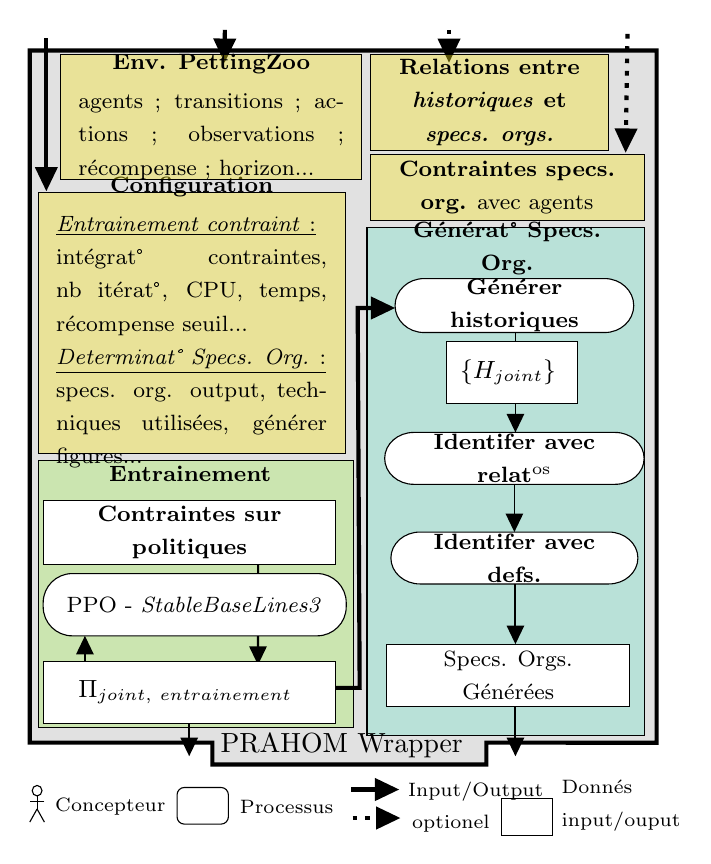
\begin{tikzpicture}[x=0.75pt,y=0.75pt,yscale=-1,xscale=1]
%uncomment if require: \path (0,1656); %set diagram left start at 0, and has height of 1656

%Straight Lines [id:da39585146483301226] 
\draw [fill={rgb, 255:red, 155; green, 155; blue, 155 }  ,fill opacity=0.3 ][line width=1.5]    (262,1077.44) -- (262,1088) -- (130,1088) -- (130,1077.44) -- (42,1077.44) -- (42,998.04) -- (42,744) -- (344,744) -- (344,1077.51) -- cycle ;
%Shape: Rectangle [id:dp15141215707199196] 
\draw  [fill={rgb, 255:red, 184; green, 233; blue, 134 }  ,fill opacity=0.54 ] (46,941.55) -- (197.88,941.55) -- (197.88,1070) -- (46,1070) -- cycle ;
%Shape: Rectangle [id:dp6360114669768389] 
\draw  [fill={rgb, 255:red, 80; green, 227; blue, 194 }  ,fill opacity=0.27 ] (204.48,829.34) -- (338,829.34) -- (338,1073.92) -- (204.48,1073.92) -- cycle ;
%Straight Lines [id:da060910289882972535] 
\draw [line width=0.75]    (118.82,1060.45) -- (118.82,1080.99) ;
\draw [shift={(118.82,1083.99)}, rotate = 270] [fill={rgb, 255:red, 0; green, 0; blue, 0 }  ][line width=0.08]  [draw opacity=0] (8.93,-4.29) -- (0,0) -- (8.93,4.29) -- cycle    ;
%Straight Lines [id:da567561296770805] 
\draw [line width=1.5]    (188.58,1051.05) -- (200.95,1051.05) -- (200,868.05) -- (214,868.05) ;
\draw [shift={(218,868.05)}, rotate = 180] [fill={rgb, 255:red, 0; green, 0; blue, 0 }  ][line width=0.08]  [draw opacity=0] (11.61,-5.58) -- (0,0) -- (11.61,5.58) -- cycle    ;
%Straight Lines [id:da27635620179975406] 
\draw [line width=0.75]    (276,1060.45) -- (276,1081) ;
\draw [shift={(276,1084)}, rotate = 270] [fill={rgb, 255:red, 0; green, 0; blue, 0 }  ][line width=0.08]  [draw opacity=0] (8.93,-4.29) -- (0,0) -- (8.93,4.29) -- cycle    ;
%Straight Lines [id:da08883699834879355] 
\draw [line width=0.75]    (276,992) -- (276,1027) ;
\draw [shift={(276,1030)}, rotate = 270] [fill={rgb, 255:red, 0; green, 0; blue, 0 }  ][line width=0.08]  [draw opacity=0] (8.93,-4.29) -- (0,0) -- (8.93,4.29) -- cycle    ;
%Straight Lines [id:da8779234517114483] 
\draw [line width=1.5]    (136,734) -- (135.88,745.84) ;
\draw [shift={(135.84,749.84)}, rotate = 270.59] [fill={rgb, 255:red, 0; green, 0; blue, 0 }  ][line width=0.08]  [draw opacity=0] (11.61,-5.58) -- (0,0) -- (11.61,5.58) -- cycle    ;
%Straight Lines [id:da43837040952509776] 
\draw [line width=1.5]  [dash pattern={on 1.69pt off 2.76pt}]  (244,734) -- (244,745.84) ;
\draw [shift={(244,749.84)}, rotate = 270] [fill={rgb, 255:red, 0; green, 0; blue, 0 }  ][line width=0.08]  [draw opacity=0] (11.61,-5.58) -- (0,0) -- (11.61,5.58) -- cycle    ;
%Shape: Ellipse [id:dp7999411998489565] 
\draw   (43.18,1100.6) .. controls (43.18,1099.21) and (44.23,1098.08) .. (45.53,1098.08) .. controls (46.83,1098.08) and (47.89,1099.21) .. (47.89,1100.6) .. controls (47.89,1101.99) and (46.83,1103.12) .. (45.53,1103.12) .. controls (44.23,1103.12) and (43.18,1101.99) .. (43.18,1100.6) -- cycle ;
%Straight Lines [id:da7827154744519647] 
\draw    (45.53,1103.12) -- (45.53,1109.43) ;
%Straight Lines [id:da757553550080027] 
\draw    (45.53,1109.43) -- (42,1115.73) ;
%Straight Lines [id:da12186027632053076] 
\draw    (45.53,1109.43) -- (49.06,1115.73) ;
%Straight Lines [id:da8177170825815439] 
\draw    (49.06,1105.64) -- (42,1105.64) ;

%Straight Lines [id:da6711978114234527] 
\draw [line width=1.5]    (196.97,1100.04) -- (215.93,1100.04) ;
\draw [shift={(219.93,1100.04)}, rotate = 180] [fill={rgb, 255:red, 0; green, 0; blue, 0 }  ][line width=0.08]  [draw opacity=0] (11.61,-5.58) -- (0,0) -- (11.61,5.58) -- cycle    ;
%Shape: Rectangle [id:dp565997856178448] 
\draw   (269.27,1104.34) -- (294,1104.34) -- (294,1122) -- (269.27,1122) -- cycle ;
%Rounded Rect [id:dp21323776879671108] 
\draw   (112.97,1102.59) .. controls (112.97,1100.64) and (114.55,1099.06) .. (116.5,1099.06) -- (134.16,1099.06) .. controls (136.11,1099.06) and (137.7,1100.64) .. (137.7,1102.59) -- (137.7,1113.18) .. controls (137.7,1115.13) and (136.11,1116.71) .. (134.16,1116.71) -- (116.5,1116.71) .. controls (114.55,1116.71) and (112.97,1115.13) .. (112.97,1113.18) -- cycle ;
%Straight Lines [id:da0858907343631472] 
\draw [line width=0.75]    (68.58,1038.32) -- (68.58,1034.8) -- (68.58,1029) ;
\draw [shift={(68.58,1026)}, rotate = 90] [fill={rgb, 255:red, 0; green, 0; blue, 0 }  ][line width=0.08]  [draw opacity=0] (8.93,-4.29) -- (0,0) -- (8.93,4.29) -- cycle    ;
%Straight Lines [id:da5873937258535422] 
\draw [line width=1.5]  [dash pattern={on 1.69pt off 2.76pt}]  (330,736) -- (329.16,789.15) ;
\draw [shift={(329.09,793.15)}, rotate = 270.91] [fill={rgb, 255:red, 0; green, 0; blue, 0 }  ][line width=0.08]  [draw opacity=0] (11.61,-5.58) -- (0,0) -- (11.61,5.58) -- cycle    ;
%Straight Lines [id:da4772036045501553] 
\draw [line width=1.5]    (50,738) -- (50,807.74) ;
\draw [shift={(50,811.74)}, rotate = 270] [fill={rgb, 255:red, 0; green, 0; blue, 0 }  ][line width=0.08]  [draw opacity=0] (11.61,-5.58) -- (0,0) -- (11.61,5.58) -- cycle    ;
%Straight Lines [id:da9532226437940816] 
\draw [line width=1.5]  [dash pattern={on 1.69pt off 2.76pt}]  (197.56,1113.77) -- (216.51,1113.77) ;
\draw [shift={(220.51,1113.77)}, rotate = 180] [fill={rgb, 255:red, 0; green, 0; blue, 0 }  ][line width=0.08]  [draw opacity=0] (11.61,-5.58) -- (0,0) -- (11.61,5.58) -- cycle    ;
%Shape: Boxed Line [id:dp7740313150184794] 
\draw [line width=0.75]    (152,988) -- (151.97,1037) ;
\draw [shift={(151.96,1040)}, rotate = 270.04] [fill={rgb, 255:red, 0; green, 0; blue, 0 }  ][line width=0.08]  [draw opacity=0] (8.93,-4.29) -- (0,0) -- (8.93,4.29) -- cycle    ;
%Straight Lines [id:da02758195492613358] 
\draw    (152,992) -- (152,1036) ;
%Straight Lines [id:da10022352286826108] 
\draw    (276,880) -- (276,884) ;
%Straight Lines [id:da39235168455073555] 
\draw    (276,914) -- (276,925) ;
\draw [shift={(276,928)}, rotate = 270] [fill={rgb, 255:red, 0; green, 0; blue, 0 }  ][line width=0.08]  [draw opacity=0] (8.93,-4.29) -- (0,0) -- (8.93,4.29) -- cycle    ;


% Text Node
\draw (225,1111) node [anchor=north west][inner sep=0.75pt]   [align=left] {{\scriptsize optionel}};
% Text Node
\draw (223,1095) node [anchor=north west][inner sep=0.75pt]   [align=left] {{\scriptsize Input/Output}};
% Text Node
\draw (297,1094) node [anchor=north west][inner sep=0.75pt]   [align=left] {{\scriptsize Donnés}\\{\scriptsize input/ouput}};
% Text Node
\draw (142,1104) node [anchor=north west][inner sep=0.75pt]   [align=left] {{\scriptsize Processus}};
% Text Node
\draw (53,1103) node [anchor=north west][inner sep=0.75pt]   [align=left] {{\scriptsize Concepteur}};
% Text Node
\draw  [fill={rgb, 255:red, 255; green, 255; blue, 255 }  ,fill opacity=1 ]  (216,988.5) .. controls (216,981.6) and (222.27,976) .. (230,976) -- (321,976) .. controls (328.73,976) and (335,981.6) .. (335,988.5) .. controls (335,995.4) and (328.73,1001) .. (321,1001) -- (230,1001) .. controls (222.27,1001) and (216,995.4) .. (216,988.5) -- cycle  ;
\draw (275.5,988.5) node   [align=left] {\begin{minipage}[lt]{78.33pt}\setlength\topsep{0pt}
\begin{center}
{\footnotesize \textbf{Identifer avec defs.}}
\end{center}

\end{minipage}};
% Text Node
\draw  [fill={rgb, 255:red, 255; green, 255; blue, 255 }  ,fill opacity=1 ]  (213,940.5) .. controls (213,933.6) and (219.27,928) .. (227,928) -- (324,928) .. controls (331.73,928) and (338,933.6) .. (338,940.5) .. controls (338,947.4) and (331.73,953) .. (324,953) -- (227,953) .. controls (219.27,953) and (213,947.4) .. (213,940.5) -- cycle  ;
\draw (275.5,940.5) node   [align=left] {\begin{minipage}[lt]{82.41pt}\setlength\topsep{0pt}
\begin{center}
{\footnotesize \textbf{Identifer avec relat}\textsuperscript{os}}
\end{center}

\end{minipage}};
% Text Node
\draw  [fill={rgb, 255:red, 255; green, 255; blue, 255 }  ,fill opacity=1 ]  (214,1030) -- (331,1030) -- (331,1060) -- (214,1060) -- cycle  ;
\draw (272.5,1045) node   [align=left] {\begin{minipage}[lt]{76.91pt}\setlength\topsep{0pt}
\begin{center}
{\footnotesize Specs. Orgs. Générées}
\end{center}

\end{minipage}};
% Text Node
\draw  [fill={rgb, 255:red, 255; green, 255; blue, 255 }  ,fill opacity=1 ]  (243,884) -- (306,884) -- (306,914) -- (243,914) -- cycle  ;
\draw (274.5,899) node   [align=left] {\begin{minipage}[lt]{40.23pt}\setlength\topsep{0pt}
\begin{center}
{\small $\displaystyle \{H_{joint}\} \ $}
\end{center}

\end{minipage}};
% Text Node
\draw  [fill={rgb, 255:red, 255; green, 255; blue, 255 }  ,fill opacity=1 ]  (218,866.87) .. controls (218,859.69) and (224.27,853.87) .. (232,853.87) -- (319,853.87) .. controls (326.73,853.87) and (333,859.69) .. (333,866.87) .. controls (333,874.05) and (326.73,879.87) .. (319,879.87) -- (232,879.87) .. controls (224.27,879.87) and (218,874.05) .. (218,866.87) -- cycle  ;
\draw (275.5,866.87) node   [align=left] {\begin{minipage}[lt]{75.66pt}\setlength\topsep{0pt}
\begin{center}
{\footnotesize \textbf{Générer historiques}}
\end{center}

\end{minipage}};
% Text Node
\draw (132.64,1072) node [anchor=north west][inner sep=0.75pt]   [align=left] {PRAHOM Wrapper};
% Text Node
\draw (272,839.45) node   [align=left] {\begin{minipage}[lt]{87.07pt}\setlength\topsep{0pt}
\begin{center}
{\footnotesize \textbf{Générat° Specs. Org.}}
\end{center}

\end{minipage}};
% Text Node
\draw  [fill={rgb, 255:red, 255; green, 255; blue, 255 }  ,fill opacity=1 ]  (48.47,1010) .. controls (48.47,1002.27) and (54.74,996) .. (62.47,996) -- (180.47,996) .. controls (188.2,996) and (194.47,1002.27) .. (194.47,1010) -- (194.47,1012) .. controls (194.47,1019.73) and (188.2,1026) .. (180.47,1026) -- (62.47,1026) .. controls (54.74,1026) and (48.47,1019.73) .. (48.47,1012) -- cycle  ;
\draw (121.47,1011) node   [align=left] {\begin{minipage}[lt]{96.56pt}\setlength\topsep{0pt}
\begin{center}
{\footnotesize PPO - \textit{StableBaseLines3}}
\end{center}

\end{minipage}};
% Text Node
\draw (119.29,947.71) node   [align=left] {\begin{minipage}[lt]{94.87pt}\setlength\topsep{0pt}
\begin{center}
{\footnotesize \textbf{Entrainement}}
\end{center}

\end{minipage}};
% Text Node
\draw  [fill={rgb, 255:red, 255; green, 255; blue, 255 }  ,fill opacity=1 ]  (48.47,960.84) -- (189.47,960.84) -- (189.47,991.84) -- (48.47,991.84) -- cycle  ;
\draw (118.97,976.34) node   [align=left] {\begin{minipage}[lt]{93.07pt}\setlength\topsep{0pt}
\begin{center}
\textbf{{\footnotesize Contraintes sur politiques}}
\end{center}

\end{minipage}};
% Text Node
\draw  [fill={rgb, 255:red, 255; green, 255; blue, 255 }  ,fill opacity=1 ]  (48.47,1038.27) -- (189.47,1038.27) -- (189.47,1068.27) -- (48.47,1068.27) -- cycle  ;
\draw (118.97,1053.27) node   [align=left] {\begin{minipage}[lt]{93.07pt}\setlength\topsep{0pt}
\begin{center}
{\small $\displaystyle \Pi _{joint,\ entrainement} \ $}
\end{center}

\end{minipage}};
% Text Node
\draw  [fill={rgb, 255:red, 248; green, 231; blue, 28 }  ,fill opacity=0.37 ]  (46,812.19) -- (194,812.19) -- (194,938.19) -- (46,938.19) -- cycle  ;
\draw (120,875.19) node   [align=left] {\begin{minipage}[lt]{97.92pt}\setlength\topsep{0pt}
\begin{center}
\textbf{{\footnotesize Configuration}}
\end{center}
{\footnotesize \underline{\textit{Entrainement contraint }:}}\\{\footnotesize intégrat° contraintes, nb itérat°, CPU, temps, récompense seuil...}\\{\footnotesize \underline{\textit{Determinat° Specs. Org.} :}}\\{\footnotesize specs. org. output, techniques utilisées, générer figures...}
\end{minipage}};
% Text Node
\draw  [fill={rgb, 255:red, 248; green, 231; blue, 28 }  ,fill opacity=0.37 ]  (206,746) -- (321,746) -- (321,792) -- (206,792) -- cycle  ;
\draw (263.5,769) node   [align=left] {\begin{minipage}[lt]{75.55pt}\setlength\topsep{0pt}
\begin{center}
\textbf{{\footnotesize Relations entre \textit{historiques }et\textit{ specs. orgs.}}}
\end{center}

\end{minipage}};
% Text Node
\draw  [fill={rgb, 255:red, 248; green, 231; blue, 28 }  ,fill opacity=0.37 ]  (206,794) -- (338,794) -- (338,826) -- (206,826) -- cycle  ;
\draw (272,810) node   [align=left] {\begin{minipage}[lt]{87.04pt}\setlength\topsep{0pt}
\begin{center}
{\footnotesize \textbf{Contraintes specs. org.} avec agents }
\end{center}

\end{minipage}};
% Text Node
\draw  [fill={rgb, 255:red, 248; green, 231; blue, 28 }  ,fill opacity=0.37 ]  (57,746) -- (202,746) -- (202,806) -- (57,806) -- cycle  ;
\draw (129.5,776) node   [align=left] {\begin{minipage}[lt]{96.07pt}\setlength\topsep{0pt}
\begin{center}
{\footnotesize \textbf{Env. PettingZoo}}
\end{center}
{\footnotesize agents ; transitions ; actions ; observations ; récompense ; horizon...}
\end{minipage}};
% Connection
\draw    (275.5,953) -- (275.5,973) ;
\draw [shift={(275.5,976)}, rotate = 270] [fill={rgb, 255:red, 0; green, 0; blue, 0 }  ][line width=0.08]  [draw opacity=0] (8.93,-4.29) -- (0,0) -- (8.93,4.29) -- cycle    ;

\end{tikzpicture}
\caption{Technical view of \emph{PRAHOM Wrapper}}
\label{fig:prahom_wrapper_technical_view}
\end{figure}

% As part of the development of the CybMASDE simulation tool,
% \footnote{\emph{Cyberdefense Multi Agent System Development Environment} is a simulator for Cyberdefense SMA available at \url{https://github.com/julien6/CybMASDE}}
\emph{PRAHOM Wrapper}\label{PettingZoo-wrapper}
\footnote{Additional information on \emph{PRAHOM Wrapper}, the examples given in this article and its developments are available at: \url{https://github.com/julien6/omarl_experiments}}
was developed as a \emph{PoC} design support tool on a PettingZoo environment by linking \textbf{histories}\footnote{A history is an n-tuple of (observation, action)} from agent to $\mathcal{M}OISE^+$ specifications. \emph{PettingZoo} is a library that offers a standard API simplifying the development of multi-agent environments and facilitates the application of MARL algorithms. An overview of the technical operation is given in \autoref{fig:prahom_wrapper_technical_view}.
%Through a case study, we propose to present the functions to extract the resulting suboptimal raw organizational specifications. Likewise during training, we present the integration of constraints on the observations received and the actions taken.

An environment
% \jp{we don't understand "these" because before you talked about "an environment"}
\emph{PettingZoo} implements the Markovian model \emph{Dec-POMDP} (Decentralized-Partially Observable Markov Decision Process)~\cite{Oliehoek2016} allowing to apply
% \jp{to apply?}
ADR techniques.
We call \textbf{solve}/\textbf{solve sub-optimally} the Dec-POMDP for a team, the search for a joint policy ($\Pi_{joint}$) allowing to maximize/exceed a cumulative reward threshold on a finite horizon (\textquote{Training} in \autoref{fig:prahom_wrapper_technical_view}). For this, the \emph{Proximal Policy Optimization} (PPO) algorithm was integrated via the \emph{Stable BaseLines3} library and taking into account possible designer constraints (by external correction, learning or modification of policies) .


To explain the joint policy, \emph{PRAHOM Wrapper} analyzes the joint histories of the $H_{joint}$ agents to generate organizational specifications. For this, several techniques are available (sequence clustering, frequency analysis, subsequence identification\dots) to which figures and supports are associated (Principal Component Analysis - PCA, dendrogram\dots)
% \jp{I think you haven't already talked about principal component analyses}.
% js: I tell myself that an ACP is something quite well known all the same...

% Based on \emph{PRAHOM Wrapper}, the \emph{PRAHOM} algorithm allows you to:
% i) \textbf{Determine organizational specifications} of $\mathcal{M}OISE^+$ by analyzing the agents' histories after (sub-optimal) resolution;
% ii) \textbf{Constrain joint policies} to those satisfying the organizational specifications of $\mathcal{M}OISE^+$.


% Indeed, a \emph{Dec-POMDP} considers several agents in a way similar to an SMA. It makes it possible to model the uncertainty of the environment for the changes induced by the actions and the observations received. Its reward function is common to agents, which promotes the formation of actions oriented towards collaboration~\cite{Beynier2013}.

% Formally, a Dec-POMDP is a 7-tuple $(S,\{A_i\},T,R,\{\Omega_i\},O,\gamma)$ , where: $S = \{s_1, . . s_{|S|}\}$ is the set of possible states; $A_{i} = \{a_{1}^{i},..,a_{|A_{i}|}^{i}\}$ the set of possible actions for the agent $i$; $T$ so that $T(s,a,s') = \probP{(s'|s,a)}$ the set of conditional transition probabilities between states; $R: S \times A \times S \rightarrow \mathbb{R}$ the reward function; $\Omega_{i} = \{o_{1}^{i},..,o_{|\Omega_{i}|}^{i}\}$ the set of observations for the agent $ag_i $ ; $O$ so that $O(s',a,o) = \probP{(o|s',a)}$ the set of conditional observation probabilities; $\gamma \in [0,1]$, the discount factor.






\subsection{Using \emph{PRAHOM Wrapper}}

\paragraph{Environment \emph{Moving Company}}

We imagined and developed the Atari game-type environment \emph{Moving Company}, an overview of which is given in \autoref{fig:env_moving_company}.
% \jp{we don't know if you invented the game or if you just implemented it as a case study}.
It consists of moving agents who must collaborate to move a package from a starting box to a final box as quickly as possible. Agents can move except in the drop-off zones (in orange on the \autoref{fig:env_moving_company}), but can pick up and drop off the package there. All observations and actions are \emph{one-hot} encoded. This environment is designed to be simple while having the advantage of bringing into play organizational mechanisms that can be evaluated manually.
%
\begin{figure}[h!]
\centering
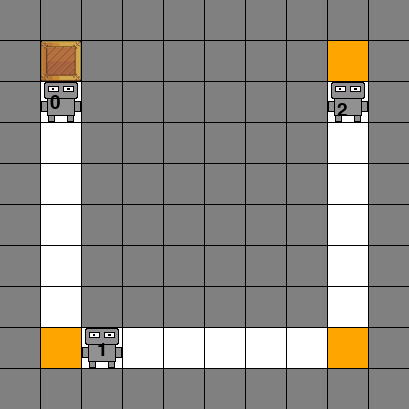
\includegraphics[width=0.154\textwidth]{figures/moving_company_1.png}
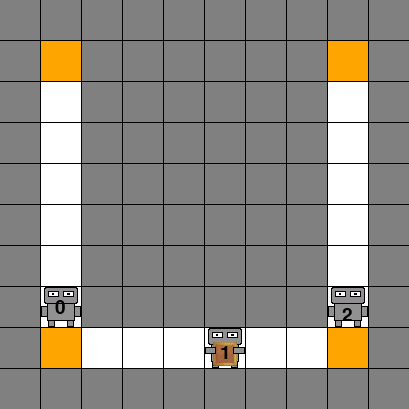
\includegraphics[width=0.154\textwidth]{figures/moving_company_2.png}
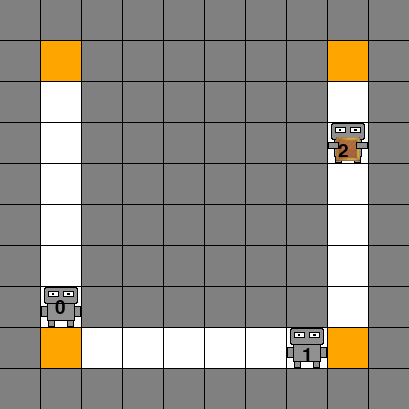
\includegraphics[width=0.154\textwidth]{figures/moving_company_3.png}
\caption{Visual renderings of \emph{Moving Company} with three moving agents and a package.}
\label{fig:env_moving_company}
\end{figure}
%
The \emph{PRAHOM Wrapper} code used for \emph{Moving Company} is summarized in \autoref{lst:wrapper_mc}.

\paragraph{Setup and configuration}

In this phase we prepare our use of \emph{PRAHOM Wrapper} (yellow boxes in \autoref{fig:prahom_wrapper_technical_view}).
After instantiating the \emph{Moving Company} environment (line 3), we define some known relationships between subhistories and known organizational specifications (line 4). Likewise we define organizational constraints (line 5). Then, \emph{PRAHOM Wrapper} wraps the environment with any relationships and pre-established constraints (line 6). Constraints and relationships can be mappings or functions to the extent that both associate an agent with its constraints and a history with known organizational specifications, respectively.

The designer can also modify the default values relating to the modes of compliance with constraints, the methods used for historical analysis, the different expected organizational specifications, and the figures and supports associated with the generated specifications.

\paragraph{Constrained training of agents}

The designer can then classically proceed with learning with the enveloped environment. Otherwise it can use the integrated PPO algorithm (green box in \autoref{fig:prahom_wrapper_technical_view}). We use this functionality (line 7) with the existing setting \textquote{PPO\_default}: an indefinite number of iterations, a learning time of 2 hours, centralized learning and decentralized execution mode, no optimization of hyper- parameters, saving the best policy and restoring from the last checkpoint if it exists.
\emph{PRAHOM Wrapper} then makes it possible to force the agents to respect the given constraint (line 5). Here, if the \textquote{agent\_0} observes that a packet is in the box higher than its own, it must take the packet (action $5$).

\paragraph{Generation and evaluation of organizational specifications}

We then generate the organizational specifications (blue box in \autoref{fig:prahom_wrapper_technical_view}) with the default profile. This generates and analyzes joint histories played over 5 episodes with the best learned policy (line 8).
\emph{PRAHOM Wrapper} takes priority into account already known relationships (line 4): if we see that the history of an agent contains the action $3$ (move left) then this agent has the role \ textquote{horizontal\_mover}.

Without a relationship between histories and pre-established organizational specifications, \emph{PRAHOM Wrapper} infers the latter based on the general definitions given. Thus, a role can be inferred by measuring similarity between histories in several complementary ways: by sequence clustering (linked to a dendrogram); by searching for the K-nearest neighbors (linked to a PCA of histories); by statistical analysis (frequency, variance of actions linked to various visualizations); etc.
Techniques are also used to infer objectives: frequency analysis of common observations of agents with the same role; analysis of recurring threshold states triggering a notable improvement in the evolution of the reward (linked to a state transition graph).

From the roles and objectives obtained, \emph{PRAHOM Wrapper} infers other organizational specifications such as compatibilities between roles, permissions and obligations. This results in the specifications specific to the organization (line 8).

\begin{lstlisting}[language=Python, caption={Synthetic use of \emph{PRAHOM Wrapper} for \emph{Moving Company}}, label={lst:wrapper_mc}]
from custom_envs.movingcompany import moving_company_v0
from prahom_wrapper import prahom_wrapper
env = moving_company_v0.parallel_env(render_mode="human")
hist_to_specs = lambda hist: {"role": "horizontal_mover"} if "3" in [act for obs, act in hist.items()] else None
agt_to_cons_specs = {"agent_0": {"[0 5 0 0 2 0 0 1 0]": 5}}
env = prahom_wrapper(env, hist_to_specs, agt_to_cons_specs, "CORRECT", ["sequence_clustering"], ["role", "goals"], ["dendogram", "PCA"])
env.train("PPO_default")
raw_specs = env.generate_specs()
\end{lstlisting}

\section{Conclusion}

\emph{PRAHOM Wrapper} provides means to constrain the learning of agents and automatically determine organizational specifications on the basis of histories, thus being agnostic of the MARL algorithm.
The current version involves the first simple statistical and unsupervised learning techniques for historical analysis to identify organizational specifications.

However, these techniques present limitations for the identification of links between roles (communications, representations) leading to incomplete specifications.
Work on hierarchical learning is likely to help characterize emerging organizations throughout learning more completely.
Ultimately, we also aim to improve the applicability of \emph{PRAHOM Wrapper} by enriching its interface and its integration in industrial and research contexts.



%%%%%%%%%%%%%%%%%%%%%%%%%%%%%%%%%%%%%%%%%%%%%%%%%%%%%%%%%%%%%%%%%%%%%%%%

%%% Use this environment to include acknowledgements (optional).
%%% This will be omitted in doubleblind mode.

\begin{ack}
    This work was supported by \emph{Thales Land Air Systems} within the framework of the \emph{Cyb'Air} chair and the \emph{AICA IWG}.
\end{ack}

%%%%%%%%%%%%%%%%%%%%%%%%%%%%%%%%%%%%%%%%%%%%%%%%%%%%%%%%%%%%%%%%%%%%%%%%

%%% Use this command to include your bibliography file.

\bibliography{references}

\end{document}
%%%%%%%%%%%%%%%%%%%%%%%%%%%%%%%%%%%%%%%%%%%%%%%%%%%%%%%%%%%%%%%%%%%%%%
